\documentclass[@BEAMER_OPTIONS@]{beamer}
    @USE_PGFPAGES@

    \usetheme[alternativetitlepage=true,titleline=true]{Torino}
    \setbeamertemplate{navigation symbols}{}
    \setbeamertemplate{note page}[plain]
    \setbeamertemplate{caption}{\insertcaption}

    \usepackage{graphicx}
    \usepackage{subfigure}
    \usepackage{xspace}
    \usepackage{adjustbox}
    \usepackage{tikz}
    \usepackage{relsize}
    \usepackage{fancyvrb}
    \fvset{fontsize=\footnotesize}
    \RecustomVerbatimEnvironment{verbatim}{Verbatim}{}
    \usepgflibrary{arrows}
    \usetikzlibrary{shadows,decorations.pathreplacing,patterns,shapes}
    \tikzstyle{every picture}=[semithick,>=stealth,remember picture]
    \usepackage{inconsolata}
    \usepackage{listings}
    \lstset{
        language=C++,
        basicstyle=\footnotesize\ttfamily,
        keywordstyle=\color{chameleon4}\bfseries,
        commentstyle=\color{chameleon1}\it\ttfamily,
        stringstyle=\color{chameleon4},
        numbers=left,
        numberstyle=\tiny,
        aboveskip=-0.02\baselineskip,
        belowskip=-0.02\baselineskip,
        columns=flexible,
        extendedchars=false,
        showstringspaces=false,
        morekeywords={global,kernel,ulong,size_t,cl_uint,cl_platform_id}
        }
    \newcommand{\code}[1]{\lstinline|#1|}
    \protected\def\plusplus{{\nolinebreak[4]\hspace{-.05em}\raisebox{.4ex}{\relsize{-3}\bf ++}}\xspace}
    \newcommand{\CXX}{{\rm C}\plusplus}
    \newcommand{\CC}{{\rm C99}\xspace}
    \newcommand{\www}[1]{\href{#1}{#1}}

    \usepackage{ifthen}
\usetikzlibrary{shadows.blur}
\newlength{\ribbonoffset}
\setlength{\ribbonoffset}{3em}

% corner, color, text
\newcommand{\ribbon}[3]{
  \ifthenelse{\equal{#1}{east}}{%
    \tikzset{ribbonrot/.style={rotate=-45}}
  }{%
    \tikzset{ribbonrot/.style={rotate=45}}
  }
  \begin{tikzpicture}[remember picture, overlay]
    \node[ribbonrot, shift={(0, -\ribbonoffset)}] at (current page.north #1) {
      \begin{tikzpicture}[remember picture, overlay,scale=0.5]
        \node[
            fill=#2,
            text centered,
            minimum width=50em,
            minimum height=1.2em,
            blur shadow,
            shadow yshift=0pt,
            shadow xshift=0pt,
            shadow blur radius=.2em,
            shadow opacity=50,
            text=white
            ](fmogh) at (0pt, 0pt) {%
            \fontfamily{phv}\selectfont\bfseries\tiny#3};
        \draw[
            white,
            dashed,
            line width=.04em,
            dash pattern=on .2em off 1.5\pgflinewidth
            ] (-25em,1em) rectangle (25em,-1em);
      \end{tikzpicture}
    };
  \end{tikzpicture}
}

    \newcommand{\forkme}{\ribbon{east}{chameleon1}{white}{\href{https://github.com/ddemidov/vexcl}{Fork me on GitHub}}}
    \newcommand{\footnoteline}{\begin{beamercolorbox}[wd=\textwidth,ht=.1ex,dp=0ex]{linemid}\end{beamercolorbox}}
    \renewcommand{\footnoterule}{\footnoteline\kern 2pt}

    \tikzset{
        treenode/.style={
            draw,
            fill=white,
            blur shadow,
            shadow xshift=1pt,
            shadow yshift=-1pt,
            shadow blur radius=2pt,
            shadow opacity=40
            }
        }


    \title{VexCL}
    \subtitle{Rapid development of scientific code for GPUs}
    \author{Denis Demidov}
    \institute{Institute of System Analysis / Russian Academy of Sciences,\\
    Kazan Federal University
    }
    \date{LPT, Toulouse, March 2018}

\begin{document}

%----------------------------------------------------------------------------
\begin{frame}{}
    \titlepage
\end{frame}

%----------------------------------------------------------------------------
\begin{frame}{VexCL~--- a vector expression template library for OpenCL/CUDA}
    \forkme

    \begin{itemize}
        \item Created for ease of \CXX based GPGPU development:
            \begin{itemize}
                \item Convenient notation for vector expressions
                \item OpenCL/CUDA JIT code generation
                \item Easily combined with existing libraries/code
                \item Header-only
            \end{itemize}
            \vspace{\baselineskip}
        \item Supported backends:
            \begin{itemize}
                \item OpenCL (Khronos \CXX bindings, Boost.Compute)
                \item NVIDIA CUDA
                \item OpenMP
                \item Maxeler FPGAs (in progress)
            \end{itemize}
            \vspace{\baselineskip}
        \item The source code is available under the MIT license:
            \begin{itemize}
                \item \href{https://github.com/ddemidov/vexcl}{https://github.com/ddemidov/vexcl}
            \end{itemize}
            \vspace{\baselineskip}
    \end{itemize}
\end{frame}

\note[itemize]{
\item VexCL is a vector expression template library for OpenCL. It allows you
    to use convenient matlab-like notation for vector operations and it
    generates the appropriate compute kernels for you automatically.
\item The library is header-only, so you don't have to build it to use it. The
    source code of the library is available on GitHub under very liberal
    MIT license.
}

%----------------------------------------------------------------------------
\begin{frame}[fragile]{Hello OpenCL}
    \begin{itemize}
        \item Compute sum of two vectors in parallel:
            \begin{itemize}
                \item \code{A} and \code{B} are large vectors.
                \item Compute \code{A = A + B}.
            \end{itemize}
            \vspace{\baselineskip}
        \item Overview of (any) OpenCL solution:
            \begin{enumerate}
                \item Initialize OpenCL context
                \item Allocate memory
                \item Transfer input data
                \item Run computations
                \item Get the results
            \end{enumerate}
    \end{itemize}
\end{frame}

\note[itemize]{
\item Let's start with a motivating example. This is classical hello world
    example for OpenCL: addition of two large vector.
\item To do anything with the OpenCL, you need to perform some standard steps,
    like context initialization, memory allocation and transfer, and the
    computations that you needed to do in the first place.
\item So let's look at how these steps are done with native OpenCL API.
}

%----------------------------------------------------------------------------
\begin{frame}[fragile]{Hello OpenCL}
    \setbeamercovered{transparent=40}
    \vspace{-1\baselineskip}
    \begin{columns}
        \begin{column}[c]{0.25\textwidth}
            \begin{exampleblock}{}
                \begin{adjustbox}{width=0.25\textwidth, height=\textheight, keepaspectratio}
                    \begin{minipage}{\textwidth}
                        \begin{uncoverenv}<1>
                            \lstinputlisting[numbers=none,linerange={1-9}]{code/hello-opencl.cpp}
                        \end{uncoverenv}
                        \begin{uncoverenv}<1,2>
                            \lstinputlisting[numbers=none,linerange={10-14}]{code/hello-opencl.cpp}
                        \end{uncoverenv}
                        \begin{uncoverenv}<1,3>
                            \lstinputlisting[numbers=none,linerange={15-33}]{code/hello-opencl.cpp}
                        \end{uncoverenv}
                        \begin{uncoverenv}<1,4>
                            \lstinputlisting[numbers=none,linerange={34-42}]{code/hello-opencl.cpp}
                        \end{uncoverenv}
                        \begin{uncoverenv}<1,5>
                            \lstinputlisting[numbers=none,linerange={43-62}]{code/hello-opencl.cpp}
                        \end{uncoverenv}
                        \begin{uncoverenv}<1,6>
                            \lstinputlisting[numbers=none,linerange={63-68}]{code/hello-opencl.cpp}
                        \end{uncoverenv}
                        \begin{uncoverenv}<1,7>
                            \lstinputlisting[numbers=none,linerange={69-71}]{code/hello-opencl.cpp}
                        \end{uncoverenv}
                        \begin{uncoverenv}<1>
                            \lstinputlisting[numbers=none,linerange={72-72}]{code/hello-opencl.cpp}
                        \end{uncoverenv}
                    \end{minipage}
                \end{adjustbox}
            \end{exampleblock}
        \end{column}
        \begin{column}[c]{0.7\textwidth}
            \begin{onlyenv}<2>
                \begin{exampleblock}{1. Query platforms}
                    \begin{adjustbox}{width=0.75\textwidth, height=\textheight, keepaspectratio}
                        \begin{minipage}{\textwidth}
                            \lstinputlisting[firstnumber=10, linerange={10-14}]{code/hello-opencl.cpp}
                        \end{minipage}
                    \end{adjustbox}
                \end{exampleblock}
            \end{onlyenv}
            \begin{onlyenv}<3>
                \begin{exampleblock}{2. Get the first available GPU}
                    \begin{adjustbox}{width=0.75\textwidth, height=\textheight, keepaspectratio}
                        \begin{minipage}{\textwidth}
                            \lstinputlisting[firstnumber=16, linerange={16-33}]{code/hello-opencl.cpp}
                        \end{minipage}
                    \end{adjustbox}
                \end{exampleblock}
            \end{onlyenv}
            \begin{onlyenv}<4>
                \begin{exampleblock}{3. Prepare and copy input data}
                    \begin{adjustbox}{width=0.75\textwidth, height=\textheight, keepaspectratio}
                        \begin{minipage}{\textwidth}
                            \lstinputlisting[firstnumber=35, linerange={35-42}]{code/hello-opencl.cpp}
                        \end{minipage}
                    \end{adjustbox}
                \end{exampleblock}
            \end{onlyenv}
            \begin{onlyenv}<5>
                \begin{exampleblock}{4. Write and compile the compute kernel}
                    \begin{adjustbox}{width=0.75\textwidth, height=\textheight, keepaspectratio}
                        \begin{minipage}{\textwidth}
                            \lstinputlisting[firstnumber=44, linerange={44-62}]{code/hello-opencl.cpp}
                        \end{minipage}
                    \end{adjustbox}
                \end{exampleblock}
            \end{onlyenv}
            \begin{onlyenv}<6>
                \begin{exampleblock}{5. Set kernel arguments and launch the computation}
                    \begin{adjustbox}{width=0.75\textwidth, height=\textheight, keepaspectratio}
                        \begin{minipage}{\textwidth}
                            \lstinputlisting[firstnumber=64, linerange={64-68}]{code/hello-opencl.cpp}
                        \end{minipage}
                    \end{adjustbox}
                \end{exampleblock}
            \end{onlyenv}
            \begin{onlyenv}<7>
                \begin{exampleblock}{6. Get the results from the compute device}
                    \begin{adjustbox}{width=0.75\textwidth, height=\textheight, keepaspectratio}
                        \begin{minipage}{\textwidth}
                            \lstinputlisting[firstnumber=70, linerange={70-71}]{code/hello-opencl.cpp}
                        \end{minipage}
                    \end{adjustbox}
                \end{exampleblock}
            \end{onlyenv}
        \end{column}
    \end{columns}
\end{frame}

\note[itemize]{
\item Here is the simplest example of using vexcl: addition of two vectors on a
    gpu card.
\item The first line is the context initialization. We provide a device filter
    to the context constructor and get all compute devices that satisfy the
    filter. Here we filter by type and get all available GPUs.
\item Data allocation and transfer is also simplified. \code{vex::vector}
    constructor allocates memory on device and possibly transfers initial data
    as well. The parameters here are list of command queues and either size or
    input host vector.
\item Line ten does what's needs to be done here. This simple expression leads
    to automatic kernel generation and launch. And then we copy the results
    back to host and see what we got.
}

%----------------------------------------------------------------------------
\begin{frame}[fragile]{Hello VexCL}
    \vspace{-1\baselineskip}
    \begin{columns}
        \begin{column}[t]{0.5\textwidth}
            \begin{exampleblock}{hello.cpp}
                \begin{adjustbox}{width=0.9\textwidth, height=\textheight, keepaspectratio}
                    \begin{minipage}{\textwidth}
                        \lstinputlisting{code/hello-vexcl.cpp}
                    \end{minipage}
                \end{adjustbox}
            \end{exampleblock}
        \end{column}
        \begin{column}[t]{0.45\textwidth}
            \begin{exampleblock}{CMakeLists.txt}
                \begin{adjustbox}{width=0.9\textwidth, height=\textheight, keepaspectratio}
                    \begin{minipage}{\textwidth}
                        \begin{lstlisting}[language=sh,
                        morekeywords={cmake_minimum_required,project,find_package,add_subdirectory,add_executable,target_link_libraries}]
cmake_minimum_required(VERSION 3.1)
project(hello)

# When VexCL is installed system wide:
find_package(VexCL)

# When VexCL is copied into a subfolder:
# add_subdirectory(vexcl)

add_executable(hello hello.cpp)
target_link_libraries(hello VexCL::OpenCL)
                        \end{lstlisting}
                    \end{minipage}
                \end{adjustbox}
            \end{exampleblock}
        \end{column}
    \end{columns}
\end{frame}

\note[itemize]{
\item Here is the simplest example of using vexcl: addition of two vectors on a
    gpu card.
\item The first line is the context initialization. We provide a device filter
    to the context constructor and get all compute devices that satisfy the
    filter. Here we filter by type and get all available GPUs.
\item Data allocation and transfer is also simplified. \code{vex::vector}
    constructor allocates memory on device and possibly transfers initial data
    as well. The parameters here are list of command queues and either size or
    input host vector.
\item Line ten does what's needs to be done here. This simple expression leads
    to automatic kernel generation and launch. And then we copy the results
    back to host and see what we got.
}

%----------------------------------------------------------------------------
\section{Interface}
\begin{frame}
    \sectionpage
\end{frame}

%----------------------------------------------------------------------------
\begin{frame}[fragile]{Initialization}
    \begin{itemize}
        \item Multi-device and multi-platform computations are supported.
        \item VexCL context is initialized from combination of device filters.
    \end{itemize}
    \vspace{-0.5\baselineskip}
    \begin{overlayarea}{\textwidth}{0.4\textheight}
    \begin{exampleblock}{Initialize VexCL context on selected devices}
        \begin{onlyenv}<1>
        \begin{lstlisting}
vex::Context ctx( vex::Filter::Any );
        \end{lstlisting}
        \end{onlyenv}
        \begin{onlyenv}<2|handout:0>
        \begin{lstlisting}
vex::Context ctx( vex::Filter::GPU );
        \end{lstlisting}
        \end{onlyenv}
        \begin{onlyenv}<3|handout:0>
        \begin{lstlisting}
vex::Context ctx(vex::Filter::Name("Intel"));
        \end{lstlisting}
        \end{onlyenv}
        \begin{onlyenv}<4|handout:0>
        \begin{lstlisting}
vex::Context ctx(vex::Filter::GPU && vex::Filter::Platform("AMD"));
        \end{lstlisting}
        \end{onlyenv}
    \end{exampleblock}
    \end{overlayarea}
    \begin{figure}
        \uncover<1,2>{
            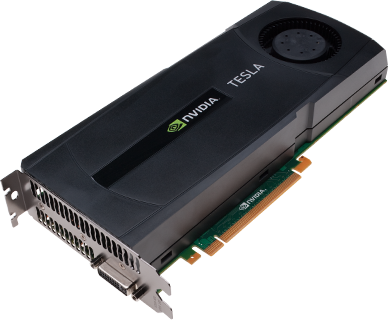
\includegraphics[width=0.2\textwidth]{tesla.png}\quad
        }
        \uncover<1,2,4>{
            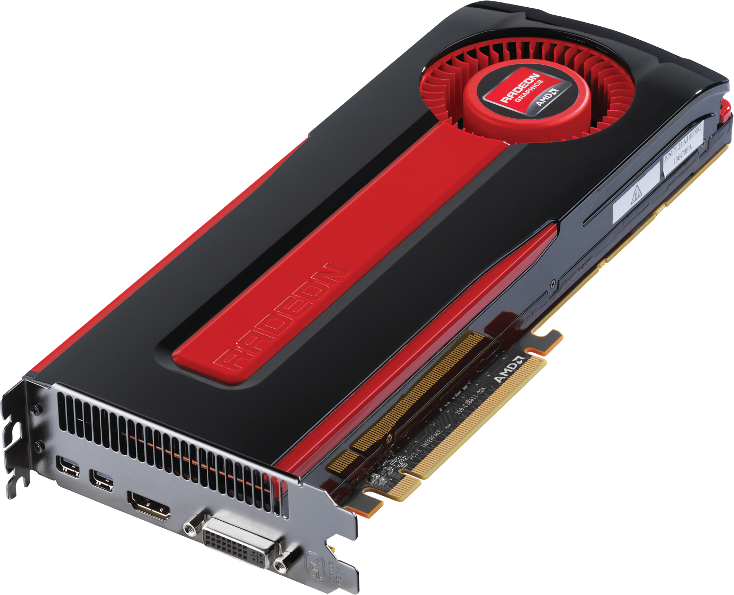
\includegraphics[width=0.2\textwidth]{radeon.png}\quad
        }
        \uncover<1,3>{
            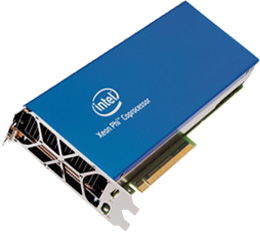
\includegraphics[width=0.17\textwidth]{intel.png}
        }
    \end{figure}
\end{frame}

\note[itemize]{
\item VexCL can transparently work with several compute devices that are
    present on your system.
\item We initialize the VexCL context with a device filter. The device filter
    is a simple functor that acts on device reference and returns a boolean
    value. Several standard filters are provided and you can write your own
    filters.
\item Let's assume that we have an NVIDIA GPU, an AMD GPU, and an Intel CPU
    installed.
    \begin{enumerate}
        \item The standard 'All' Filter select any device available, so we end
            with three devices in our context.
        \item If we want to select only GPUs, then we can filter the devices by
            type.
        \item It is also possible to combine the device filters with logical
            operators.  Here we select a GPU that is provided by AMD OpenCL
            platform.
        \item And here is an example of a custom filter. Here it selects any
            device that has at least 4GB of memory.
    \end{enumerate}
}

%----------------------------------------------------------------------------
\begin{frame}[fragile]{Memory and work splitting}
    \setbeamercovered{transparent=40}
    \begin{exampleblock}{}
        \begin{onlyenv}<1|handout:0>
        \begin{lstlisting}
vex::Context ctx( vex::Filter::Count(1) );
        \end{lstlisting}
        \end{onlyenv}
        \begin{onlyenv}<2|handout:0>
        \begin{lstlisting}
vex::Context ctx( vex::Filter::GPU );
        \end{lstlisting}
        \end{onlyenv}
        \begin{onlyenv}<3>
        \begin{lstlisting}
vex::Context ctx( vex::Filter::DoublePrecision );
        \end{lstlisting}
        \end{onlyenv}
        \begin{uncoverenv}<1>
        \begin{lstlisting}[firstnumber=last]

vex::vector<double> x(ctx, N);
vex::vector<double> y(ctx, N);

x = vex::element_index() * (1.0 / N);
y = sin(2 * x) + sqrt(1 - x * x);
        \end{lstlisting}
        \end{uncoverenv}
    \end{exampleblock}
    \setbeamercovered{invisible}
    \begin{figure}
        \begin{tikzpicture}
            \draw (0,2.5) rectangle +(8,0.1);
            \draw (0,2.5) grid[step=0.1] +(8,0.1);
            \draw (-0.3,2.6) node{x};

            \draw (0,2.0) rectangle +(8,0.1);
            \draw (0,2.0) grid[step=0.1] +(8,0.1);
            \draw (-0.3,2.1) node[anchor=center]{y};

            \uncover<1-3> {
            \draw (1,0.5) node{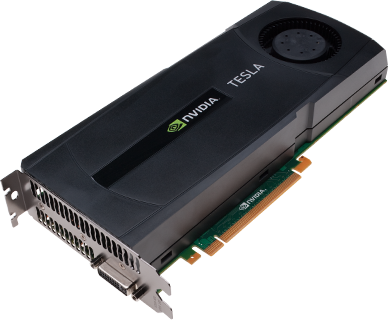
\includegraphics[width=0.2\textwidth]{tesla.png}};
            }

            \uncover<2-3> {
            \draw (4,0.5) node{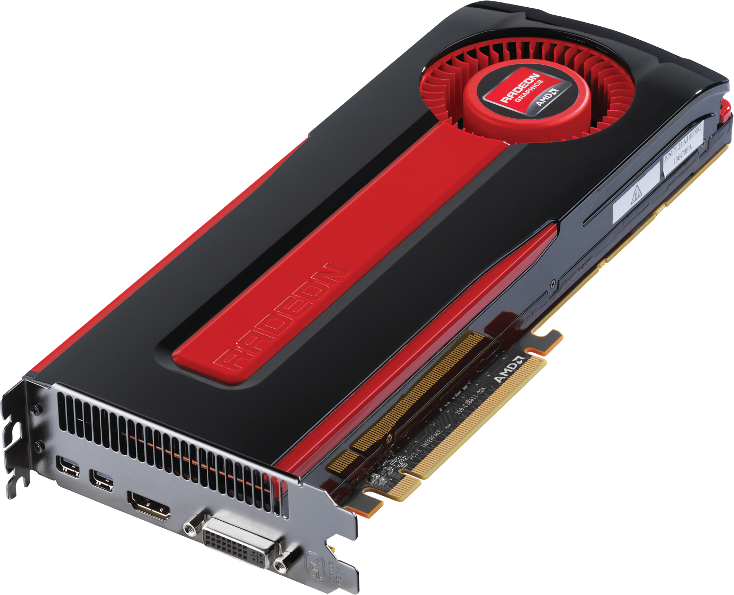
\includegraphics[width=0.2\textwidth]{radeon.png}};
            }

            \uncover<3> {
            \draw (7.5,0.5) node{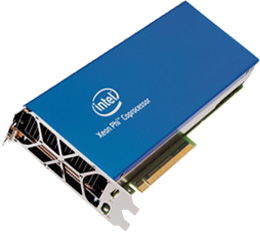
\includegraphics[width=0.17\textwidth]{intel.png}};
            }

            \uncover<1|handout:0> {
            \draw[->,chameleon3,style=dashed] (0,2.7) -- (0,1.8)
                .. controls +(east:0.5) and +(north west:0.5) ..
                (1.4,1.5);
            \draw[->,chameleon3,style=dashed] (8,2.7) -- (8,1.8)
                .. controls +(west:0.5) and +(north east:0.5) ..
                (1.6,1.5);
            }

            \uncover<2|handout:0> {
            \draw[->,chameleon3,style=dashed] (0,2.7) -- (0,1.8)
                .. controls +(east:0.5) and +(north west:0.5) ..
                (1.4,1.5);
            \draw[->,chameleon3,style=dashed] (4,2.7) -- (4,1.8)
                .. controls +(west:0.5) and +(north east:0.5) ..
                (1.6,1.5);

            \draw[->,chameleon3,style=dashed] (4,2.7) -- (4,1.8)
                .. controls +(east:0.1) and +(north west:0.2) ..
                (4.4,1.5);
            \draw[->,chameleon3,style=dashed] (8,2.7) -- (8,1.8)
                .. controls +(west:0.5) and +(north east:0.5) ..
                (4.6,1.5);
            }

            \uncover<3> {
            \draw[->,chameleon3,style=dashed] (0,2.7) -- (0,1.8)
                .. controls +(east:0.5) and +(north west:0.5) ..
                (1.4,1.5);
            \draw[->,chameleon3,style=dashed] (3,2.7) -- (3,1.8)
                .. controls +(west:0.5) and +(north east:0.5) ..
                (1.6,1.5);

            \draw[->,chameleon3,style=dashed] (3,2.7) -- (3,1.8)
                .. controls +(east:0.5) and +(north west:0.2) ..
                (4.4,1.5);
            \draw[->,chameleon3,style=dashed] (6,2.7) -- (6,1.8)
                .. controls +(west:0.5) and +(north east:0.5) ..
                (4.6,1.5);

            \draw[->,chameleon3,style=dashed] (6,2.7) -- (6,1.8) -- (7.4,1.5);
            \draw[->,chameleon3,style=dashed] (8,2.7) -- (8,1.8) -- (7.6,1.5);
            }
        \end{tikzpicture}
    \end{figure}
\end{frame}

\note[itemize]{
\item Now that we know how to initialize VexCL context, let's see how device
    vectors are allocated.
\item Here we allocate three vectors, and initialize two of them with
    constant values.
\item Each vector receives a list of queues at initialization.  Since each
    queue corresponds to a specific device, vectors know where to put their
    data to.
    \begin{enumerate}
        \item For example, if we only have the Tesla card in our context, then
            it will hold the complete memory for all of our vectors.
        \item If we use both of the available GPUs, then the vectors will be
            split between the devices. This split is by default proportional to
            the GPU bandwidth and is guaranteed to be consistent for vectors of
            the same size. This consistency allows VexCL to run computations
            independently on all devices in context.
        \item If we add the CPU to the context, it will get smaller share of
            the data and arithmetic operations.
    \end{enumerate}
\item Care must be taken with the use of several devices. VexCL tries to split
    the memory as fair as it can, but it is probable that your program will
    run at the speed of the slowest device.
}

%----------------------------------------------------------------------------
\begin{frame}[fragile]{Copies between host and device memory}
    \begin{exampleblock}{}
        \begin{lstlisting}
vex::vector<double> d(ctx, n);
std::vector<double> h(n);
double a[100];
        \end{lstlisting}
    \end{exampleblock}
    \vspace{\baselineskip}
    \begin{columns}
        \begin{column}{0.5\textwidth}
            \begin{exampleblock}{STL-like range copies}
                \begin{lstlisting}
vex::copy(d.begin(), d.end(), h.begin());
vex::copy(d.begin(), d.begin() + 100, a);
                \end{lstlisting}
            \end{exampleblock}
        \end{column}
        \begin{column}{0.4\textwidth}
            \begin{exampleblock}{Simple copies}
                \begin{lstlisting}
vex::copy(d, h);
vex::copy(h, d);
                \end{lstlisting}
            \end{exampleblock}
        \end{column}
    \end{columns}
    \vspace{\baselineskip}
    \begin{columns}
        \begin{column}{0.5\textwidth}
            \begin{exampleblock}{Map OpenCL buffer to host pointer}
                \begin{lstlisting}
auto p = d.map(devnum);
std::sort(&p[0], &p[d.part_size(devnum)]);
                \end{lstlisting}
            \end{exampleblock}
        \end{column}
        \begin{column}{0.4\textwidth}
            \begin{exampleblock}{Access single element (\emph{slow})}
                \begin{lstlisting}
double v = d[42];
d[0] = 0;
                \end{lstlisting}
            \end{exampleblock}
        \end{column}
    \end{columns}
\end{frame}

\note[itemize]{
\item Copies between host and device memory may be done with simple copy
    function that copy the complete vector either way,
\item or, if you need to do partial copy, you can use STL-like syntax.
\item Vectors also overload array subscript operator, so you can have direct
    read or write access to any element of a vector. But this should be used
    with caution because it is slow. The intended use for this is a single
    element access or debugging.
\item Data may also be accessed through iterators, so it is possible to use,
    for example, an STL algorithm with device vector as a temporary solution.
}

%----------------------------------------------------------------------------
\begin{frame}[fragile]{What vector expressions are supported?}
    \begin{itemize}
        \item All vectors in an expression have to be \emph{compatible}:
            \begin{itemize}
                \item Have same size
                \item Located on same devices
            \end{itemize}
        \item What may be used:
            \begin{columns}
                \begin{column}{0.4\textwidth}
                    \begin{itemize}
                        \item Vectors, scalars, constants
                        \item Arithmetic, logical operators
                        \item Built-in functions
                        \item User-defined functions
                        \item Random number generators
                        \item Slicing and permutations
                    \end{itemize}
                \end{column}
                \begin{column}{0.42\textwidth}
                    \begin{itemize}
                        \item Reduce to a scalar (sum, min, max)
                        \item Reduce across chosen dimensions
                        \item Stencil operations
                        \item Sparse matrix~-- vector products
                        \item Fast Fourier Transform
                        \item Sort, scan, reduce by key
                    \end{itemize}
                \end{column}
            \end{columns}
    \end{itemize}
\end{frame}

\note[itemize]{
\item So, what kind of expressions can you use in VexCL?
\item First, any vectors used in an expression have to be compatible.
\item If this requirement is satisfied, then expressions may combine
    vectors and scalars with almost any binary operators. OpenCL math functions
    and user-defined functions are also available.
}

%----------------------------------------------------------------------------
\begin{frame}[fragile]{Builtin operations and functions}
    \begin{columns}
        \begin{column}{0.38\textwidth}
            \begin{exampleblock}{This expression:}
                \begin{lstlisting}
x = 2 * y - sin(z);
                \end{lstlisting}
            \end{exampleblock}
        \end{column}
        \begin{column}{0.55\textwidth}
            \begin{itemize}
                \item \code{export VEXCL_SHOW_KERNELS=1}\\
                    to see the generated code.
            \end{itemize}
        \end{column}
    \end{columns}
    \begin{exampleblock}{\ldots results in this kernel:}
        \begin{lstlisting}
kernel void vexcl_vector_kernel(
    ulong n,
    global double * prm_1,
    int prm_2,
    global double * prm_3,
    global double * prm_4
)
{
    for(size_t idx = get_global_id(0); idx < n; idx += get_global_size(0)) {
        prm_1[idx] = ( ( prm_2 * prm_3[idx] ) - sin( prm_4[idx] ) );
    }
}
        \end{lstlisting}
    \end{exampleblock}
    \begin{tikzpicture}[overlay,scale=0.6]
        \draw (16,8) node(sub)[draw,fill=white,ellipse,drop shadow]{$-$};

        \draw (sub) +(-2.00,-1) node(mul)[draw,fill=white,drop shadow,ellipse]{$*$};
        \draw (sub) +( 2.00,-1) node(sin)[draw,fill=white,drop shadow,ellipse]{sin};
        \draw (mul) +(-2.00,-1) node(two)[draw,fill=white,drop shadow,minimum size=0.5cm]{2};
        \draw (mul) +( 2.00,-1) node(y)  [draw,fill=white,drop shadow,minimum size=0.5cm]{y};
        \draw (sin) +( 1.75,-1) node(z)  [draw,fill=white,drop shadow,minimum size=0.5cm]{z};

        \draw (sub) -- (mul);
        \draw (sub) -- (sin);
        \draw (mul) -- (two);
        \draw (mul) -- (y);
        \draw (sin) -- (z);
    \end{tikzpicture}
\end{frame}

\note{ }

%----------------------------------------------------------------------------
\begin{frame}[fragile]{User-defined functions}
    \begin{exampleblock}{Defining a function:}
        \begin{lstlisting}
VEX_FUNCTION( double, sqr, (double, x)(double, y),
    return x * x + y * y;
    );
        \end{lstlisting}
    \end{exampleblock}
    \begin{exampleblock}{Using the function:}
        \begin{lstlisting}
Z = sqrt( sqr(X, Y) );
        \end{lstlisting}
    \end{exampleblock}
\end{frame}

\note[itemize]{
\item It is possible to define an OpenCL function that may be used with vector
    expressions. You need to provide function body, parameter types, and return
    type.
\item Function body has to be of \code{extern const char} type, to allow it's
    use as a template parameter. And it has to be defined at global scope.
\item Inside the body function parameters are always named prm1, prm2, etc.
\item Here we define 'between' function that returns true if it's second
    parameter is between it's first and third parameters. The UserFunction
    object is stateless, so it may be good idea to define it at global scope
    as well, next to it's body.
\item Now we may use the function in expressions. Any vector expression may be
    used as a parameter for a user-defined (or builtin) function.
}

%----------------------------------------------------------------------------
\begin{frame}[fragile]{User functions are translated to OpenCL functions}
    \begin{exampleblock}{}
        \begin{lstlisting}
Z = sqrt( sqr(X, Y) );
        \end{lstlisting}
    \end{exampleblock}
    \begin{exampleblock}{\ldots gets translated to:}
        \begin{lstlisting}
double sqr(double x, double y) {
    return x * x + y * y;
}

kernel void vexcl_vector_kernel(
    ulong n,
    global double * prm_1,
    global double * prm_2,
    global double * prm_3
)
{
    for(size_t idx = get_global_id(0); idx < n; idx += get_global_size(0)) {
        prm_1[idx] = sqrt( sqr( prm_2[idx], prm_3[idx] ) );
    }
}
        \end{lstlisting}
    \end{exampleblock}
    \begin{tikzpicture}[overlay,scale=0.6]
        \draw (16,8.75) node(sqrt)[draw,fill=white,ellipse,drop shadow]{sqrt};

        \draw (sqrt) +(0.00,-2) node(sqr)[draw,fill=white,ellipse,drop shadow]{sqr};

        \draw (sqr) +(-2.00,-1) node(x) [draw,fill=white,drop shadow,minimum size=0.5cm]{x};
        \draw (sqr) +( 2.20,-1) node(y) [draw,fill=white,drop shadow,minimum size=0.5cm]{y};

        \draw (sqrt) -- (sqr);
        \draw (sqr)  -- (x);
        \draw (sqr)  -- (y);
    \end{tikzpicture}
\end{frame}

\note{ }

%----------------------------------------------------------------------------
\begin{frame}[fragile]{Random number generation}
    \begin{itemize}
        \item VexCL provides\footnote{Contributed by
            \href{https://github.com/neapel}{Pascal Germroth}
            $\langle$\href{mailto:pascal@ensieve.org}{pascal@ensieve.org}$\rangle$}
            \emph{counter-based} random number generators from
            Random123\footnote{D. E. Shaw Research,
                \href{http://www.deshawresearch.com/resources\_random123.html}{http://www.deshawresearch.com/resources\_random123.html}}
            suite.
            \begin{itemize}
                \item The generators are \emph{stateless}; mixing functions are
                    applied to element indices.
                \item Implemented families: \code{threefry} and \code{philox}.
                \item Both pass TestU01/BigCrush; up to \alert{$2^{64}$}
                    independent streams with a period of \alert{$2^{128}$}.
                \item Performance: \alert{$\approx 10^{10}$}~Samples/sec (Tesla
                    K20c).
            \end{itemize}
        \item \code{vex::Random<T,G>}~--- uniform distribution.
        \item \code{vex::RandomNormal<T,G>}~--- normal distribution.
    \end{itemize}
    \begin{exampleblock}{}
        \begin{lstlisting}
vex::Random<double> rnd;
vex::vector<double> x(ctx, n);

x = rnd(vex::element_index(), std::rand());
        \end{lstlisting}
    \end{exampleblock}
\end{frame}

\note[itemize]{
\item Random number generation is a useful feature that is used often in, e.g.,
    molecular dynamics.
\item Random number generators in VexCL are stateless, so they don't require
    additional storage or global memory interactions. Randomness is obtained by
    applying mixing functions to element indices.
}

%----------------------------------------------------------------------------
\begin{frame}[fragile]{Reductions}
    \begin{itemize}
        \item Class \code{vex::Reductor<T, kind>} allows to reduce arbitrary
            \emph{vector expression} to a\\ single value of type \code{T}.
        \item Supported reduction kinds: \code{SUM}, \code{SUM_Kahan},
            \code{MIN}, \code{MAX}
    \end{itemize}
    \begin{exampleblock}{Inner product}
        \begin{lstlisting}
vex::Reductor<double, vex::SUM> sum(ctx);
double s = sum(x * y);
        \end{lstlisting}
    \end{exampleblock}
    \begin{exampleblock}{Number of elements in x between 0 and 1}
        \begin{lstlisting}
vex::Reductor<size_t, vex::SUM> sum(ctx);
size_t n = sum( (x > 0) && (x < 1) );
        \end{lstlisting}
    \end{exampleblock}
    \begin{exampleblock}{Maximum distance from origin}
        \begin{lstlisting}
vex::Reductor<double, vex::MAX> max(ctx);
double d = max( sqrt(x * x + y * y) );
        \end{lstlisting}
    \end{exampleblock}
\end{frame}

\note[itemize]{
\item Reduction is an operation of reducing a vector to a single value.
\item The most frequent types are summation and finding minimum or maximum
    element of a vector.
\item VexCL provides Reductor functor that accepts any valid vector expression
    as a parameter.
\item For example, to compute an inner product of two vectors we compute sum of
    their elementwise product.
\item To find number of elements in vector x that are greater than zero and
    less than one, we compute sum of the corresponding boolean expression.
\item And to find the maximum distance from axis origin for a set of
    two-dimensional points, we compute exactly that: max of their radius.
}

%----------------------------------------------------------------------------
\begin{frame}[fragile]{Sparse matrix~-- vector products}
    \begin{itemize}
        \item Class \code{vex::sparse::matrix<T>} holds representation of a
            sparse matrix on compute devices.
        \item Constructor accepts matrix in common CRS format:
            \begin{itemize}
                \item row indices, columns and values of nonzero entries.
            \end{itemize}
    \end{itemize}
    \begin{exampleblock}{Construct matrix}
        \begin{lstlisting}
vex::sparse::matrix<double> A(ctx, n, n, ptr, col, val);
        \end{lstlisting}
    \end{exampleblock}

    \begin{exampleblock}{Compute residual value}
        \begin{lstlisting}[firstnumber=last]
// vex::vector<double> u, f, r;
r = f - A * u;
double res = max( fabs(r) );
        \end{lstlisting}
    \end{exampleblock}
\end{frame}

\note[itemize]{
\item Sparse matrix -- vector operation is also provided. A matrix is imported
    from commonly used compressed row storage format.
\item Note that matrix-vector product is not a first-class citizen in vector
    expressions. It uses neighbor values; and neighbors may reside on a
    different compute device. So extra work is needed to exchange data between
    devices. That is why matrix-vector products may only be used in additive
    expressions.
}

%----------------------------------------------------------------------------
\begin{frame}[fragile]{Raw pointer arithmetic}
    \begin{itemize}
        \item \code{raw_pointer(const vector<T>&)} function returns pointer to
            vector's data\\ inside vector expression.
            \begin{itemize}
                \item May be used to implement complex access patterns.
            \end{itemize}
    \end{itemize}
    \begin{exampleblock}{1D Laplace operator:}
        \begin{lstlisting}[keepspaces=true]
auto ptr   = vex::raw_pointer(x);
auto idx   = vex::element_index();

auto left  = if_else(idx > 0,     i - 1, i);
auto right = if_else(idx + 1 < n, i + 1, i);

y = 2 * ptr[idx] - ptr[left] - ptr[right];\end{lstlisting}
    \end{exampleblock}
\end{frame}

\note{ }

%----------------------------------------------------------------------------
\begin{frame}[fragile]{N-body problem with raw pointers}
    \begin{equation*}
        y_i = \sum_{j \neq i} e^{-|x_i - x_j|}
    \end{equation*}
    \begin{exampleblock}{}
        \begin{lstlisting}
VEX_FUNCTION(double, nbody, (size_t, n)(size_t, i)(double*, x),
    double sum = 0, myval = x[i];
    for(size_t j = 0; j < n; ++j)
        if (j != i) sum += exp(-fabs(x[j] - myval));
    return sum;
    );

y = nbody(x.size(), vex::element_index(), raw_pointer(x));
        \end{lstlisting}
    \end{exampleblock}
\end{frame}

\note{ }

%----------------------------------------------------------------------------
\section{Usage examples}
\begin{frame}
    \sectionpage
\end{frame}

%----------------------------------------------------------------------------
\begin{frame}[fragile]{Monte Carlo $\pi$}
    \vspace{-1\baselineskip}
    \begin{columns}
        \begin{column}{0.55\textwidth}
            \begin{itemize}
                \item Compute approximate value of $\pi$:
            \end{itemize}
            \vspace{\baselineskip}
            \begin{equation*}
                \frac{\text{area of circle}}{\text{area of square}} =
                \frac{\pi r^2}{(2r)^2} = \frac{\pi}{4},
            \end{equation*}
            \begin{equation*}
                \pi = 4 \frac{\text{area of circle}}{\text{area of square}}
                \approx 4 \frac{\operatorname{count}(\text{\color{chameleon4}{points
                in circle}})}{\operatorname{count}(\text{\color{chameleon4}{all}
                \color{chameleon3}{points}})}
            \end{equation*}
        \end{column}
        \begin{column}{0.35\textwidth}
            \begin{figure}
                \includegraphics[width=\textwidth]{mcpi}
            \end{figure}
        \end{column}
    \end{columns}
    \begin{exampleblock}{}
        \begin{lstlisting}[texcl=true]
vex::Random<cl_double2> rnd; // Generates 2D points in $[0,1]\times[0,1]$
vex::Reductor<size_t, vex::SUM> sum(ctx);

double pi = 4.0 * sum( length( rnd(vex::element_index(0, n), seed) ) < 1 ) / n;
        \end{lstlisting}
    \end{exampleblock}
\end{frame}

\note[itemize]{
\item Here is a bit more complex example of what you can do with VexCL.
\item Imagine we want to compute an approximate value of $\pi$ with Monte-Carlo
    method. We can use the following equalities to do this.
}

%----------------------------------------------------------------------------
\begin{frame}[fragile]{Monte Carlo $\pi$: the generated kernel}
    \begin{columns}
        \begin{column}[t]{0.2\textwidth}
            \begin{exampleblock}{}
                \begin{adjustbox}{width=0.30\textwidth, height=\textheight, keepaspectratio}
                    \begin{minipage}{\textwidth}
                        \lstinputlisting[numbers=none,linerange={1-50}]{code/pi-kernel.cpp}
                    \end{minipage}
                \end{adjustbox}
            \end{exampleblock}
        \end{column}
        \begin{column}[t]{0.2\textwidth}
            \begin{exampleblock}{}
                \begin{adjustbox}{width=0.30\textwidth, height=\textheight, keepaspectratio}
                    \begin{minipage}{\textwidth}
                        \lstinputlisting[numbers=none,linerange={51-100}]{code/pi-kernel.cpp}
                    \end{minipage}
                \end{adjustbox}
            \end{exampleblock}
        \end{column}
        \begin{column}[t]{0.2\textwidth}
            \begin{exampleblock}{}
                \begin{adjustbox}{width=0.30\textwidth, height=\textheight, keepaspectratio}
                    \begin{minipage}{\textwidth}
                        \lstinputlisting[numbers=none,linerange={101-150}]{code/pi-kernel.cpp}
                    \end{minipage}
                \end{adjustbox}
            \end{exampleblock}
        \end{column}
        \begin{column}[t]{0.3\textwidth}
            \begin{exampleblock}{}
                \begin{adjustbox}{width=0.30\textwidth, height=\textheight, keepaspectratio}
                    \begin{minipage}{\textwidth}
                        \lstinputlisting[numbers=none,linerange={151-200}]{code/pi-kernel.cpp}
                    \end{minipage}
                \end{adjustbox}
            \end{exampleblock}
        \end{column}
    \end{columns}
\end{frame}

\note{}

%----------------------------------------------------------------------------
\begin{frame}{Solving ODEs on GPUs}
    \vspace{-1\baselineskip}
    \begin{columns}
        \begin{column}{0.5\textwidth}
            \begin{block}{Lorenz attractor system}
                \vspace{-1\baselineskip}
                \begin{align*}
                    \dot{x} &= -\sigma \left( x - y \right), \\
                    \dot{y} &= R x - y - xz, \\
                    \dot{z} &= -bz + xy.
                    \label{eq:lorenz}
                \end{align*}
            \end{block}
        \end{column}
        \begin{column}{0.4\textwidth}
            \begin{figure}
                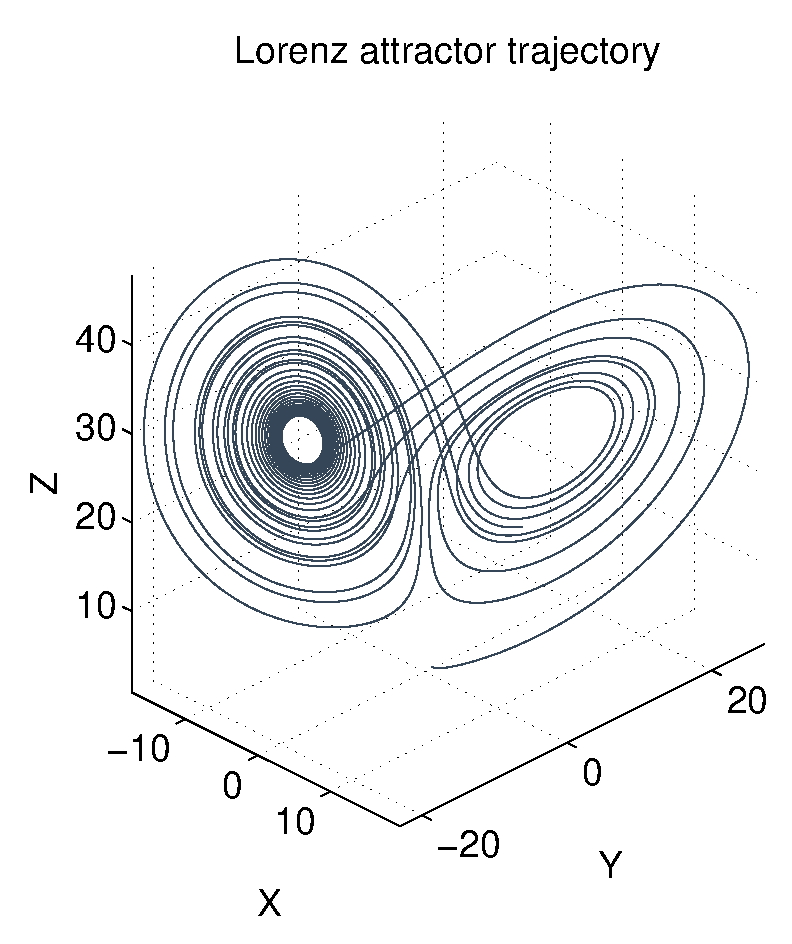
\includegraphics[width=\textwidth]{lorenz}
            \end{figure}
        \end{column}
    \end{columns}
    \begin{itemize}
        \item Parameter study for the Lorenz attractor system:
            \begin{itemize}
                \item Solve large number of Lorenz systems, each
                    for a different value of $R$.
                \item Let's use Boost.odeint together with VexCL
                    for that.
            \end{itemize}
    \end{itemize}
    \footnoteline
    \begin{footnotesize}
        \begin{itemize}
            \item[{[1]}] K. Ahnert, D. Demidov, and M. Mulansky.  Solving
                ordinary differential equations on GPUs.\\
                In \emph{Numerical Computations with GPUs} (pp. 125-157).
                Springer, 2014.
                \href{http://dx.doi.org/10.1007/978-3-319-06548-9\_7}{doi:10.1007/978-3-319-06548-9\_7}
        \end{itemize}
    \end{footnotesize}
\end{frame}

%----------------------------------------------------------------------------
\begin{frame}{Using Boost.odeint}
    \begin{block}{Generic ODE:}
        \begin{gather*}
            \frac{\mbox{d} x}{\mbox{d} t } = \dot{x} = f(x , t),\\
             x(0) = x_0.
        \end{gather*}
    \end{block}

    \vspace{\baselineskip}

    \begin{exampleblock}{Using Boost.odeint:}
        \begin{itemize}
            \item Define state type (what is $x$?)
            \item Choose integration method
            \item Provide system function (define $f(x,t)$)
            \item Integrate over time
        \end{itemize}
    \end{exampleblock}
\end{frame}

%----------------------------------------------------------------------------
\begin{frame}[fragile]{Implementation}
    \setbeamercovered{transparent=40}
    \vspace{-1\baselineskip}
    \begin{columns}
        \begin{column}[c]{0.35\textwidth}
            \begin{exampleblock}{}
                \begin{adjustbox}{width=0.42\textwidth, height=\textheight, keepaspectratio}
                    \begin{minipage}{\textwidth}
                        \begin{uncoverenv}<1>
                            \lstinputlisting[numbers=none,linerange={1-7}]{code/lorenz.cpp}
                        \end{uncoverenv}
                        \begin{uncoverenv}<1,2>
                            \lstinputlisting[numbers=none,linerange={8-14}]{code/lorenz.cpp}
                        \end{uncoverenv}
                        \begin{uncoverenv}<1,3>
                            \lstinputlisting[numbers=none,linerange={15-26}]{code/lorenz.cpp}
                        \end{uncoverenv}
                        \begin{uncoverenv}<1,4>
                            \lstinputlisting[numbers=none,linerange={27-45}]{code/lorenz.cpp}
                        \end{uncoverenv}
                    \end{minipage}
                \end{adjustbox}
            \end{exampleblock}
        \end{column}
        \begin{column}[c]{0.62\textwidth}
            \begin{onlyenv}<2>
                \begin{exampleblock}{1. State type and stepper type}
                    \begin{adjustbox}{width=0.75\textwidth, height=\textheight, keepaspectratio}
                        \begin{minipage}{\textwidth}
                            \lstinputlisting[firstnumber=9, linerange={9-14}]{code/lorenz.cpp}
                        \end{minipage}
                    \end{adjustbox}
                \end{exampleblock}
            \end{onlyenv}
            \begin{onlyenv}<3>
                \begin{exampleblock}{2. System function}
                    \begin{adjustbox}{width=0.73\textwidth, height=\textheight, keepaspectratio}
                        \begin{minipage}{\textwidth}
                            \lstinputlisting[firstnumber=10, linerange={16-26}]{code/lorenz.cpp}
                        \end{minipage}
                    \end{adjustbox}
                \end{exampleblock}
            \end{onlyenv}
            \begin{onlyenv}<4>
                \begin{exampleblock}{3. Integrate}
                    \begin{adjustbox}{width=0.75\textwidth, height=\textheight, keepaspectratio}
                        \begin{minipage}{\textwidth}
                            \lstinputlisting[firstnumber=27, linerange={28-45}]{code/lorenz.cpp}
                        \end{minipage}
                    \end{adjustbox}
                \end{exampleblock}
            \end{onlyenv}
        \end{column}
    \end{columns}
\end{frame}

%----------------------------------------------------------------------------
\begin{frame}[fragile]{Performance}{NVIDIA Tesla K40c, Intel Core i7 920
    \vspace{0.25\baselineskip}}
    \begin{figure}
        \includegraphics[width=0.9\textwidth]{perf}
    \end{figure}
\end{frame}

%----------------------------------------------------------------------------
\begin{frame}[fragile]{Summary}
    \begin{columns}
        \begin{column}{0.65\textwidth}
            \begin{itemize}
                \item VexCL allows to write compact and readable code.
                    \begin{itemize}
                        \item It's great for fast prototyping of scientific
                            GPGPU applications.
                            \vspace{0.5\baselineskip}
                        \item The performance is often on-par with manually
                            written kernels.
                            \vspace{0.5\baselineskip}
                        \item \emph{Using custom kernels or third-party
                            functionality is still possible.}
                    \end{itemize}
                    \vspace{\baselineskip}
                    \pause
                \item It stresses the compiler greatly.
                    \begin{itemize}
                        \item Compilation takes a lot of RAM and a lot of
                            time.
                        \item But, it's easy to combine \CXX with Python:
                            \www{http://pybind11.readthedocs.io}
                    \end{itemize}
            \end{itemize}
        \end{column}
        \begin{column}{0.3\textwidth}
            \begin{uncoverenv}<2>
                \begin{figure}
                    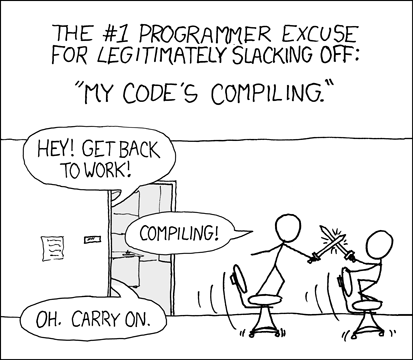
\includegraphics[width=\textwidth]{compiling.png}
                    \caption{\tiny \www{https://xkcd.com/303/}}
                \end{figure}
            \end{uncoverenv}
        \end{column}
    \end{columns}
\end{frame}

%----------------------------------------------------------------------------
\begin{frame}[fragile]{Creating python bindings for \CXX with pybind11}
    \setbeamercovered{transparent=40}
    \vspace{-0.5\baselineskip}
    \begin{columns}
        \begin{column}[c]{0.3\textwidth}
            \begin{exampleblock}{}
                \begin{adjustbox}{width=0.28\textwidth, height=\textheight, keepaspectratio}
                    \begin{minipage}{\textwidth}
                        \begin{uncoverenv}<1>
                            \lstinputlisting[numbers=none, linerange={1-10}]{code/pylorenz.cpp}
                        \end{uncoverenv}
                        \begin{uncoverenv}<1,2>
                            \lstinputlisting[numbers=none, linerange={11-17}]{code/pylorenz.cpp}
                        \end{uncoverenv}
                        \begin{uncoverenv}<1,3>
                            \lstinputlisting[numbers=none, linerange={18-22}]{code/pylorenz.cpp}
                        \end{uncoverenv}
                        \begin{uncoverenv}<1,4>
                            \lstinputlisting[numbers=none, linerange={23-52}]{code/pylorenz.cpp}
                        \end{uncoverenv}
                        \begin{uncoverenv}<1,5>
                            \lstinputlisting[numbers=none, linerange={53-67}]{code/pylorenz.cpp}
                        \end{uncoverenv}
                    \end{minipage}
                \end{adjustbox}
            \end{exampleblock}
        \end{column}
        \begin{column}[c]{0.6\textwidth}
            \begin{onlyenv}<2>
                \begin{exampleblock}{1. State type and stepper type}
                    \begin{adjustbox}{width=0.78\textwidth, height=\textheight, keepaspectratio}
                        \begin{minipage}{\textwidth}
                            \lstinputlisting[firstnumber=12, linerange={12-17}]{code/pylorenz.cpp}
                        \end{minipage}
                    \end{adjustbox}
                \end{exampleblock}
            \end{onlyenv}
            \begin{onlyenv}<3>
                \begin{exampleblock}{2. Context initialization}
                    \begin{adjustbox}{width=0.75\textwidth, height=\textheight, keepaspectratio}
                        \begin{minipage}{\textwidth}
                            \lstinputlisting[firstnumber=19, linerange={19-22}]{code/pylorenz.cpp}
                        \end{minipage}
                    \end{adjustbox}
                \end{exampleblock}
            \end{onlyenv}
            \begin{onlyenv}<4>
                \begin{exampleblock}{3. System function}
                    \begin{adjustbox}{width=0.6\textwidth, height=\textheight, keepaspectratio}
                        \begin{minipage}{\textwidth}
                            \lstinputlisting[firstnumber=24, linerange={24-52}]{code/pylorenz.cpp}
                        \end{minipage}
                    \end{adjustbox}
                \end{exampleblock}
            \end{onlyenv}
            \begin{onlyenv}<5>
                \begin{exampleblock}{4. Python bindings}
                    \begin{adjustbox}{width=0.78\textwidth, height=\textheight, keepaspectratio}
                        \begin{minipage}{\textwidth}
                            \lstinputlisting[firstnumber=54, linerange={54-67}]{code/pylorenz.cpp}
                        \end{minipage}
                    \end{adjustbox}
                \end{exampleblock}
            \end{onlyenv}
        \end{column}
    \end{columns}
\end{frame}

%----------------------------------------------------------------------------
\begin{frame}[fragile]{Calling \CXX code from Python}
    \begin{exampleblock}{}
        \begin{lstlisting}[language=python]
import pylorenz as lorenz

n = 32   # Number of parameters
m = 500  # Length of trajectory

# Parameters
R = linspace(0.1, 10, n)
sigma = 10.0
b = 8/3

# Initial solution
S = empty((m, 3, n))
S[0,:,:] = 10.0

# Integration
ode = lorenz.Stepper(sigma, b, R)
for i in range(1,m):
    S[i] = ode.advance(S[i-1], 1, 0.01)
        \end{lstlisting}
    \end{exampleblock}
\end{frame}

%----------------------------------------------------------------------------
\begin{frame}{Projects using VexCL}
    \begin{description}[\quad]
        \item[AMGCL] --- an efficient, flexible, and extensible Algebraic
            Multigrid implementation:
            \begin{itemize}
                \item \www{https://github.com/ddemidov/amgcl}
            \end{itemize}
        \item[Boost.odeint] --- numerical solution of Ordinary Differential
            Equations:
            \begin{itemize}
                \item \www{https://github.com/boostorg/odeint}
            \end{itemize}
        \item[Antioch] --- A New Templated Implementation Of Chemistry for
            Hydrodynamics\\(The University of Texas at Austin):
            \begin{itemize}
                \item \www{https://github.com/libantioch/antioch}
            \end{itemize}
        \item[FDBB] --- Fluid Dynamics Building Blocks (\raisebox{-0.04\baselineskip}{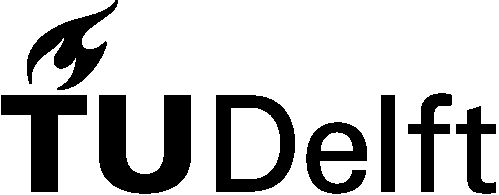
\includegraphics[height=\baselineskip]{tudelft.pdf}}):
            \begin{itemize}
                \item \www{https://gitlab.com/mmoelle1/FDBB}
            \end{itemize}
    \end{description}
\end{frame}

\note{ }

%----------------------------------------------------------------------------
\begin{frame}{}
    \begin{description}[Documentation:]
        \item[Source code:] \www{https://github.com/ddemidov/vexcl}
            \vspace{\baselineskip}
        \item[Documentation:] \www{http://vexcl.readthedocs.io}
            \vspace{\baselineskip}
        \item[Slides:] \www{https://speakerdeck.com/ddemidov}
            \vspace{\baselineskip}
        \item[Example codes:] \www{https://github.com/ddemidov/vexcl-talks}
    \end{description}
\end{frame}

\end{document}
